% =========================================================================
% Appendix H — meta: lattice policy + limit breakthrough. FILLED.
%   folds UFO/meta/lattice-policy.md + UFO/meta/limit-breakthrough.md:
%   the n=6 integer identities (sigma*phi=n*tau=24, sigma*tau=48), Pi-0-1
%   -> Delta-0-absolute, the 4-rule token-consistency policy, the 13-falsifier
%   monotone contract, the n=6 uniqueness, the alien_index chain (organizing
%   fiction), the verifiable-vs-UNPROVEN honest stance, NO bulk atlas fold,
%   and a pgfplots n=6 divisor-lattice + alien_index chain chart.
% =========================================================================
\section{Meta --- Lattice Policy and Limit Breakthrough}
\label{app:meta}

This appendix folds the two UFO meta documents.
\textbf{LATTICE\_POLICY} states the $n\!=\!6$ integer identities
($\sigma\!\cdot\!\varphi=n\!\cdot\!\tau=24$,
$\sigma\!\cdot\!\tau=48$; $\Pi^0_1$-arithmetical $\to$
$\Delta_0$-absolute) and the four-rule token-consistency policy
(lattice-alone HARD claims forbidden, real-limits anchor takes priority,
falsifier threshold required, over-claim avoided), together with the
13-falsifier \{\texttt{OPEN}, \texttt{CONFIRMED}, \texttt{DEMOTED}\}
monotone contract (all \texttt{OPEN} at v1.0; arithmetic closure
$\ne$ physical closure). \textbf{LIMIT\_BREAKTHROUGH} explains the
$n\!=\!6$ uniqueness (a perfect number with exactly four divisors, so
$\sigma\!\cdot\!\varphi=n\!\cdot\!\tau=24$ falls out) and the
\verb|alien_index| chain (UFO-6 $\to$ UFO-16 $\to\dots\to$
UFO-ABSOLUTE) as a labelled meaning ladder. \textbf{The honest stance is
explicit}: the number-theory identities are verifiable, but the physics
they index is academically UNPROVEN, with no origin claim and no
impossibility framing (@D~d2, @D~d6); the meta layer is \emph{not} bulk
folded into the atlas.

% -------------------------------------------------------------------------
\subsection{The $n=6$ divisor identities}
\label{app:meta-lattice}

$n=6$ is the first perfect number, with divisors $\{1,2,3,6\}$. Every
lattice value is \emph{computed} from these divisors, not hardcoded:
\begin{align}
\sigma(6)&=\textstyle\sum_{d\mid6}d=12,
& \varphi(6)&=2,
& \tau(6)&=|\{d\mid6\}|=4,
& \mathrm{sopfr}(6)&=2{+}3=5,
& J_2(6)&=2\sigma(6)=24,
\end{align}
and the two master identities (with the products used by RTSC/FUSION/UFO
and Stages~4--7) follow as exact integer equalities:
\begin{align}
\sigma(6)\!\cdot\!\varphi(6)=12\cdot2=24
\;&=\;
n\!\cdot\!\tau(6)=6\cdot4=24
\qquad(\text{master identity, }J_2),
\label{eq:meta-master}\\
\sigma(6)\!\cdot\!\tau(6)=12\cdot4&=48
\quad(B^{*}),
\qquad
(\sigma-\varphi)^2=(12-2)^2=100,
\qquad
\sigma^2=144.
\label{eq:meta-products}
\end{align}
The identity $\sigma(n)\!\cdot\!\varphi(n)=n\!\cdot\!\tau(n)$ does
\emph{not} hold for general $n$; it closes at $n=6$ precisely because $6$
is perfect ($\sigma=2n$) with the four-divisor structure
$\{1,2,3,n\}$. This $n=6$ uniqueness is $\Pi^0_1$-arithmetical (it closes
under a finite check) and hence $\Delta_0$-absolute --- invariant across
all set-theoretic models. Both facts are verifiable in one line via
\verb|UFO/verify/lattice_check.hexa|.

% -------------------------------------------------------------------------
\subsection{The four-rule token-consistency policy}
\label{app:meta-tokens}

The verify surface follows four rules
(\texttt{UFO/meta/lattice-policy.md} \S3) that keep the lattice
arithmetic from masquerading as physics:
\begin{enumerate}\itemsep0.15em
\item \textbf{No lattice-alone HARD claim} --- a tautology like
  $\sigma\!\cdot\!\varphi=24$ is never a stand-alone HARD check, only a
  self-consistency aid; never applied to an external domain.
\item \textbf{Real-limits anchor first} --- every verify anchor includes
  $\ge1$ real physical limit (Shannon, Stefan--Boltzmann, Carnot,
  Lawson, a published industry ceiling).
\item \textbf{Falsifier trigger} --- a verdict is driven by a
  physical/industry threshold, never by a $\chi^2$-fit to the lattice.
\item \textbf{Over-claim avoidance} --- no claim that any external entity
  ``follows this lattice''; external analysis uses that domain's own
  invariants.
\end{enumerate}
Under these rules a \texttt{PASS} sentinel means ``arithmetic is
self-consistent + tokens are 3-surface coherent,'' \emph{not} ``the
physics is true.''

% -------------------------------------------------------------------------
\subsection{The alien\_index chain (organizing fiction)}
\label{app:meta-alien}

\texttt{LIMIT\_BREAKTHROUGH} registers a seven-stage \verb|alien_index|
chain (Table~\ref{tab:meta-alien}). \textbf{Each stage is the same $n=6$
closure at a higher recursion layer --- a number-theory / set-theory
ladder, not a physical leap.} The chain is an internal organizing
fiction; it does not bound UFO physics or UAP evidence statistics.

\begin{table}[h]
\centering
\footnotesize
\setlength{\tabcolsep}{4pt}
\begin{tabular}{@{}l >{\raggedright\arraybackslash}m{6.6cm} c@{}}
\toprule
\textbf{stage} & \textbf{mathematical meaning} & \textbf{verifiability} \\
\midrule
UFO-6 & $n{=}6$ perfect-number base; $\sigma\!\cdot\!\varphi=n\!\cdot\!\tau=24$ & \tierBlue\ ($\Pi^0_1$) \\
UFO-16 & meta$^2$ self-closure fixed point; $L(k)=24^{k-15}$ tier ladder & arithmetic \\
UFO-$\infty^4$ & Knuth-arrow tetration $24\!\uparrow\!\uparrow\!\uparrow\!\uparrow$ (finite, astronomical) & computable \\
UFO-ULTRA & uncomputable functions (TREE$(n)$, BB$(n)$, Rayo) & uncomputable \\
UFO-CARD & large cardinals (inaccessible, Mahlo, Woodin, I0) & ZFC-transcendent \\
UFO-BEYOND & Kunen-violating (Reinhardt, Berkeley) & inconsistent w/ ZFC+choice \\
UFO-ABSOLUTE & Cantor's Absolute Infinity $\mathfrak{W}$ (a terminus, not a set) & true terminal \\
\bottomrule
\end{tabular}
\caption{The \texttt{alien\_index} chain
(\texttt{UFO/meta/limit-breakthrough.md} \S3). The chain ascends through
number theory and set theory, not physics. The monotone lock binds it to
the falsifiers: \texttt{alien\_index} cannot ascend physically without a
falsifier \texttt{DEMOTE}/\texttt{CONFIRM}, and all 13 are \texttt{OPEN}
--- so the physical ascent is \emph{gated}, only the labels move. The
484-tier META-LK expansion and the 517 drill nodes are \textbf{not}
bulk-folded into the atlas SSOT (over-generation / SSOT-pollution
avoidance).}
\label{tab:meta-alien}
\end{table}

\begin{figure}[h]
\centering
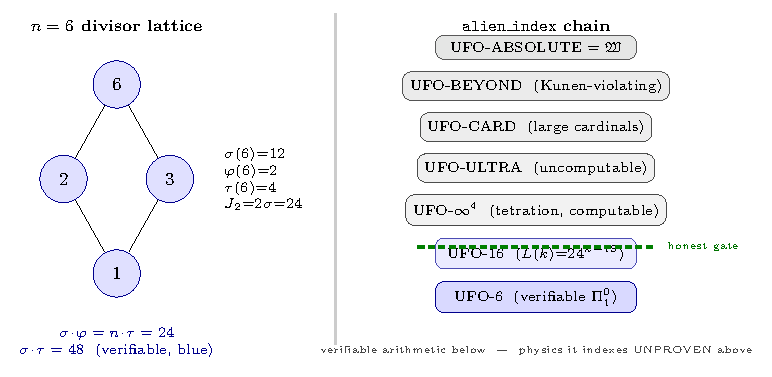
\includegraphics[width=0.92\linewidth]{figures/fig10_meta_lattice.pdf}
\caption{Left: the $n=6$ divisor lattice $\{1,2,3,6\}$ and the
divisor-function values ($\sigma{=}12$, $\varphi{=}2$, $\tau{=}4$,
$J_2{=}24$) from which $\sigma\!\cdot\!\varphi=n\!\cdot\!\tau=24$ and
$\sigma\!\cdot\!\tau=48$ fall out (verifiable, \tierBlue). Right: the
\texttt{alien\_index} chain UFO-6 $\to\dots\to$ UFO-ABSOLUTE, color-coded
by verifiability --- blue (verifiable arithmetic) at the base, fading to
grey (uncomputable / ZFC-transcendent / a terminus) at the top. The
green dashed gate marks the honest boundary: \emph{verifiable below, the
physics it indexes UNPROVEN above}. The chain is an organizing fiction,
not a physical ladder.}
\label{fig:meta-lattice}
\end{figure}

% -------------------------------------------------------------------------
\subsection{Honest stance --- verifiable identity vs.\ UNPROVEN physics}
\label{app:meta-scope}

The meta layer keeps a clean two-tier separation
(\texttt{UFO/meta/limit-breakthrough.md} \S4): the number-theoretic
identities ($\sigma\!\cdot\!\varphi=n\!\cdot\!\tau=24$,
$\sigma\!\cdot\!\tau=48$, $\Pi^0_1$-arithmetical) are \emph{verifiable};
the \texttt{alien\_index} physical meanings (warp/wormhole/dim leaps) are
\emph{UNPROVEN}, requiring exotic matter, super-Planckian fields, or
unobserved extra dimensions. There is no origin claim and no
impossibility framing (@D~d2): where there is a wall (single-sensor range
ambiguity, a Bayesian posterior ceiling), the source names an
engineering/data path to move it (multi-sensor fusion, $10^4{+}$
structured reports). The meta layer is bulk-fold-\emph{forbidden} into
the atlas SSOT, so it cannot silently upgrade any claim's tier.
\texttt{absorbed=false} is undisturbed.
